\begin{Figure}[h]
\begin{center}
\unitlength1cm

\begin{picture}(14.0,5.0)
\psfrag{E1}[c][c]{${\bf E}_1$}
\psfrag{E2}[c][c]{${\bf E}_2$}
\psfrag{E3}[c][c]{${\bf E}_3$}
\psfrag{e1}[c][c]{${\bf e}_1$}
\psfrag{e2}[c][c]{${\bf e}_2$}
\psfrag{e3}[c][c]{${\bf e}_3$}
\psfrag{B}[c][c]{${\cal B}$}
\psfrag{S}[c][c]{${\cal S}$}
\psfrag{X}[c][c]{${\bf X}$}
\psfrag{x}[c][c]{${\bf x}$}
\psfrag{M}[c][c]{${\bf M}$}
\psfrag{L}[c][c]{${\BLambda}$}
\psfrag{F}[c][c]{${\bf F}$}
\psfrag{phi}[c][c]{$\Bvarphi_t({\bf X})$}
\put(1.5,0){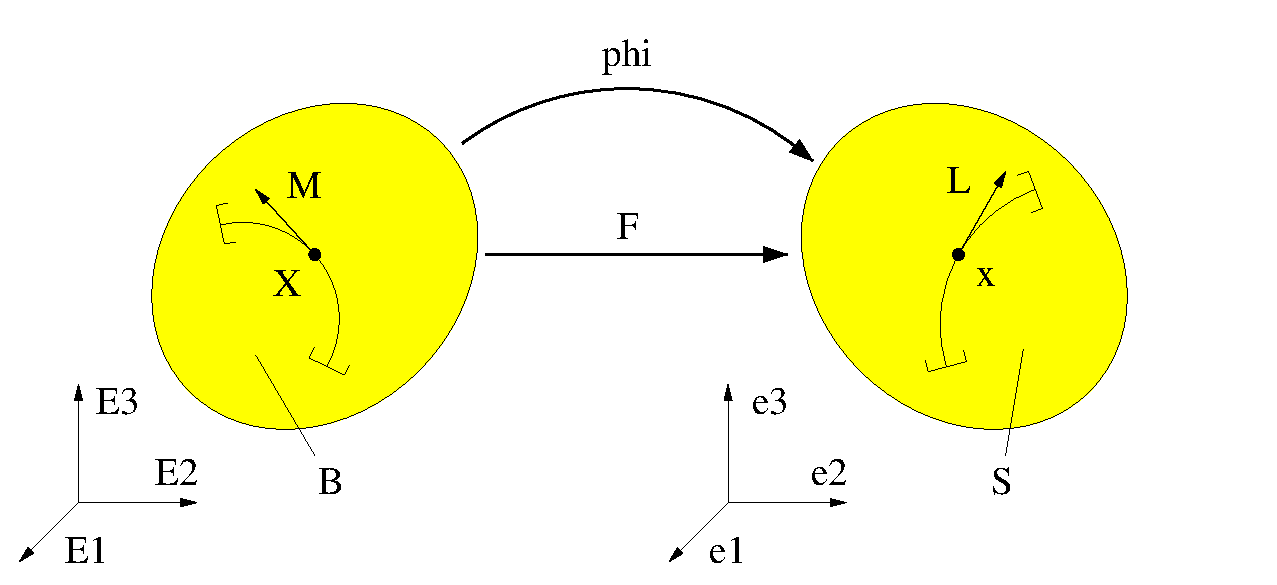
\includegraphics[width=0.75\textwidth]{\dir/config1.eps}}
\end{picture}

\setlength{\baselineskip}{11pt}
\caption{Abbildung der Referenzkonfiguration $\B$ auf die
         Momentankonfiguration ${\cal S}$ mit der nichtlinearen
         Deformationsabbildung $\Bvarphi_t $.
} \label{fig2_01}
\end{center}
\end{Figure}%

%%% Local Variables: 
%%% mode: latex
%%% TeX-master: "sec"
%%% End: 
